\documentclass[11pt]{article}
\usepackage{geometry} % see geometry.pdf on how to lay out the page. There's lots.
\usepackage{hyperref}
\usepackage{graphicx}
\usepackage{gensymb}
\usepackage[affil-it]{authblk}
\usepackage[toc,page]{appendix}
\usepackage{pifont}
\usepackage{amsmath}
\usepackage{amssymb}
\usepackage{relsize}
\usepackage{draftwatermark}
\usepackage[mathscr]{eucal}

\SetWatermarkText{DRAFT}
\SetWatermarkScale{6}
\SetWatermarkLightness{0.95}

\renewcommand{\min}{\expandafter\,\operatorname*{min}}
\renewcommand{\max}{\expandafter\,\operatorname*{max}}

% \geometry{letter} % or letter or a5paper or ... etc
% \geometry{landscape} % rotated page geometry

% See the ``Article customise'' template for come common customisations

\title{An Explanation of Calibration-Free Pulse Oximetry}
\author{Robert L. Read
  \thanks{read.robert@gmail.com}
}
\affil{Founder, Public Invention, an educational non-profit.}


\date{\today}

%%% BEGIN DOCUMENT
\begin{document}

\maketitle

%% \tableofcontents

\section{Introduction}

This is an attempt to clarify the ideas presented by Chugh and Kaur\cite{ChughAndKaur2015}.

A valuble resource for understanding pulse oximetry in general is available at HowEquipmentWorks.com\cite{howPulseOx}.

The EWB-Austin Instrumentation group is hoping to teach the world how to construct a practical pulse oximeter inexpensively to provide
the medical benefits of pulse oximetry to parts of the world where it is not presently widespread. To do this, it must be understandable
and inexpensive.

We have breadboarded simple equipment and analyzed signals with an Arudino Uno, constituting a very simple pulse oximeter.

Chugh and Kaur\cite{ChughAndKaur2015} have presented a theoretical approach to constructing a pulse oximeter that does not require calibration.
If a pulse oximeter could be made withot calibration, this would be a large advantage for anyone in a developing country attempting to construct
and use one correctly.

Chugh and Kaur\cite{ChughAndKaur2015} cite and build upon earlier works \cite{harini2014design}, which attempts to do hardware filtering
and equalization of the signals. Both of these works cite a seminal work by Reddy et al. \cite{reddy2009novel}.

I believe all three of these papers have serious flaws. This paper is my attempt to explain this, mostly to myself. It
is not ready to consider a critique of those papers.

I assert that \cite{reddy2009novel}, while valuable, is flawed or at least very confusing in its attempt to use ``slope'' of voltage against
time, when clearly removing time from that analysis would be clearer. The means of deriving Figure 6 in that table is either incorrect or
not explained.

Chugh and Kaur\cite{ChughAndKaur2015} cannot be correct as written, as it is clearly the case that differences in sensor sensitivities
would affect their results, in my interpretation. Furthermore, that papers defines the quantity $R$ in equations 1, 8, and 12, in ways
which are mutually inconsistent (unless, very confusingly, they intent R to mean different quantities in these cases.

Note: Nitzan\cite{nitzan2014pulse} is much clearer, giving a similar equation for $SaO2$ 
fundamental equation based on the standard $R$ ``ratio of ratios'', roughly matching these papers.


\section{Review of Chugh and Kaur}

Chugh and Kaur\cite{ChughAndKaur2015} paper is concise, but not perfectly clear to us upon first reading. We here work through some of the
math they present in order to verify it and to verify that we correctly understand it.

In section $1.i$, the paper restates the Beer-Lambert law\cite{wiki:Beer-Lambert} as:

\begin{equation}
  A = \ln \frac{I_o}{I_t} = \varepsilon \cdot C \cdot L
  \end{equation}

where $A$ is the absorbance, $\varepsilon$ is the wavelength-dependent extinction\footnote{Note that Wikipedia\cite{wiki:MolarAttenuation} states the IUPAC discourages the
term {\emph extinction coefficient} in favor of {\emph molar attunation coefficient}.}
coeffecint, $C$ is the concentration of the absorbing material present in the
path and $L$ is the path length.


Using Wolframalpha.com to check this, we see that this formulation
(with a change of variable names)
is indeed just a restatement of the Beer-Lambert law as expressed by the
Wikipedia article\cite{wiki:Beer-Lambert}, although it seems that the computation
of the absorbance from the incident and transmitted light via 
logarithm should be, according to Wikipedia, base 10:

\begin{equation}
  A = \log_{10} \frac{I_o}{I_t} = \varepsilon \cdot C \cdot L
\end{equation}


Chugh and Kaur state the multi-species version of the Beer-Lambert law,
and then state the absorbance at the two distinct wavelenghts at which
oxygenated hemoglobin and deoxygenated hemoglobin differ maximally,
which they call $RED$ and $IR$, in terms of the concentrations of
two species (oxygenated ($C_{hbo}$) and
deoxygenated  ($C_{hb}$)).

\begin{equation}
  A_{RED} = (\varepsilon_{hbo(red)}\cdot C_{hbo} + \varepsilon_{hb(red)}\cdot C_{hb}) \cdot L
\end{equation}

\begin{equation}
  A_{IR} = (\varepsilon_{hbo(IR)}\cdot C_{hbo} + \varepsilon_{hb(IR)}\cdot C_{hb}) \cdot L
\end{equation}

The then define the ration $R$ as the ratio of the absorbance measured
at these wavelengths:

\begin{equation}
  R = \frac{A_{RED}}{A_{IR}}
  \end{equation}

Using straightforward algebra, R becomes independent of the path length $L$:
\begin{equation}
  R = \frac{(\varepsilon_{hbo(red)}\cdot C_{hbo} + \varepsilon_{hb(red)}\cdot C_{hb})}{(\varepsilon_{hbo(IR)}\cdot C_{hbo} + \varepsilon_{hb(IR)}\cdot C_{hb})}
\end{equation}

Using straightforward algebra, they rearrange this:
\begin{equation}
  \label{eq:chb}
  C_{hb} = C_{hbo} \frac{R \cdot \varepsilon_{hbo(IR)} - \varepsilon_{hbo(red)}}
  {\varepsilon_{hb(red)} - R \cdot \varepsilon_{hb(IR)} }
\end{equation}

Note: Chugh and Kaur use slightly different variable names than used at Wikipedia.
Possibly in this paper we will change the names yet again to make them more
conformant to that style.

They then define $SpO_2$ (periphereal oxygen saturation)
\cite{wiki:SpO2,wiki:oxygensaturation}:
\begin{equation}
  \label{eq:spo2}
  SpO_2 = \frac{C_{hbo}}{C_{hbo} + C_{hb}}
\end{equation}

Then the substitute \ref{eq:chb} into \ref{eq:spo2} and simplify:
\begin{equation}
  SpO_2 = \frac{100 (\varepsilon_{hbo(red)} - R \cdot \varepsilon_{hb(IR)})}
  {(\varepsilon_{hb(red)} - \varepsilon_{hbo(red)}) + R \cdot(\varepsilon_{hbo(IR)} - \varepsilon_{hb(IR)})}
\end{equation}

The then claim that R can be computed by taking the base-10 log of that AC 
component of the $RED$ and $IR$ signals.

I believe they paper suggests this to be the the difference between the the maximum
of the time-varying signal and the minimum of the time-varying signal.

(Only an electrical engineer would understand the term ``AC component'' to
mean the time-varying signal. I believe a better terminology is the
``pulsative signal''. This is the part of the signal remaining when the
unvarying signal is removed. In terms of the FFT, the very low frequencies
of the signal may be removed (those lower than the lowest human pulse, which
is about 0.5 Hz).)

However, the absolute difference between the greatest and least
transmittance (and inversely absorbance) is highly dependent on the
machinery and physical body measured.

Define the ``Pulsative Absorbance'' at frequency $\lambda$. 
\begin{equation}
  P_{\lambda} = \frac{\text{max of moving average of absorbance}}
  {\text{min of moving average of absorbance }}
\end{equation}

Where the absorbance is computed by the definition:
\begin{equation}
 A_{\lambda} = \log_{10} \frac{I_{\lambda o}}{I_{\lambda t}}   
\end{equation}

If we make the reasonable assumption that $I_t$ is proportional
to our our measured signal, then we can substitute and
remove the dependence ont he intensity of the transmitted light:
\begin{equation}
  P_{\lambda} = \frac{\max{A_{\lambda}}}
  {\min{A_{\lambda}}}
\end{equation}

So we can create the ratio of the blood-full absorbance
to the ratio of the blood-empty absorbance:
\begin{equation}
  P_{\lambda} = \frac{\max{A_{\lambda}}}
  {\min{A_{\lambda}}}
\end{equation}




Can it be that they mean the ratio of the pulsative part of the signal
to the non-pulsative part of the signal?  This is the change in
the absorbance.



\section{Finding Peak-to-Peak Values: A novel algorithm}

Using this approach, a fundamental need it so measure the peak-to-peak difference of
the time-varying part of the signal. This can be accomplished by keeping a running
maximum and a running minimum.

On October 28th, I had coded an approach to this that works.  I was not
able to find a good algorithm for the Aduino.

Additional, I believe I have discovered a new algorithm that will
be effective for the Arduino, with a constant running time and
extremely good performance with a constant amount of space.

I have not yet coded this algorithm. This is my attempt to record my thoughts.

\subsection{DROPBORINGLIN: A fast constant space algorithm for the running maximum of a sampled signal }

Douglas \cite{douglas1996running} provides a good algorithm {\em MAXLIST} for computing a
running maximum. This algorithm builds upon his observation that one may
keep an ordered list of potential maxima.

In order to produce a constant space algorithm with good error
characteristics, we define {\em DROPBORINGLIN} whose fundamental insight
is that we can define a ring buffer of constant size to keep the samples.
If the signal is not monotone decreasing, the observation {\em MAXLIST} observation
tells us that only a small number of samples need be stored, as they tend
to be higher than, and therefore obviate, older samples.

However, if the signal is monotone decreasing, to be perfect we might
have to keep every sample, which cannot be done in small space.

Therefore we observe that the error produced by dropping an individual
sample varies, and is easily computed. If we ignore the fact that
we are dealing with  digital signal processing series which is probably
a sampling of a smooth waveform, we can compute this area as two right triangles.

However, we can do even better if we assume that our time series is coming
from a samples series of limited frequency, and that therefore if the window
slides over a sample in time the maximum should not abruptly change, but is
better appxoimated by a linear interpolation.

Each of the samples which is not either the newest or the oldest can
then be thought of as giving us information about how far away
the signal is from a linear interpolation between the preceding and
succeeding samples. Some samples are more surpsising than others,
in that they are further away from this linear interpolation. We
propose that the best way to compute the maximum in limited space
is to drop the sample that is the ``most boring''. Since this
is easily computed for each sample, we have a simple algorithm that
operates in constant space. When the signal is monotone decreasing,
the algorithm may be erroneous, but will only be erroneous by
an amount which we can can bound and minimize.

This algorithm is particularly well-suited to implementation on an Arduino,
where memory is limited.

\begin{figure}
  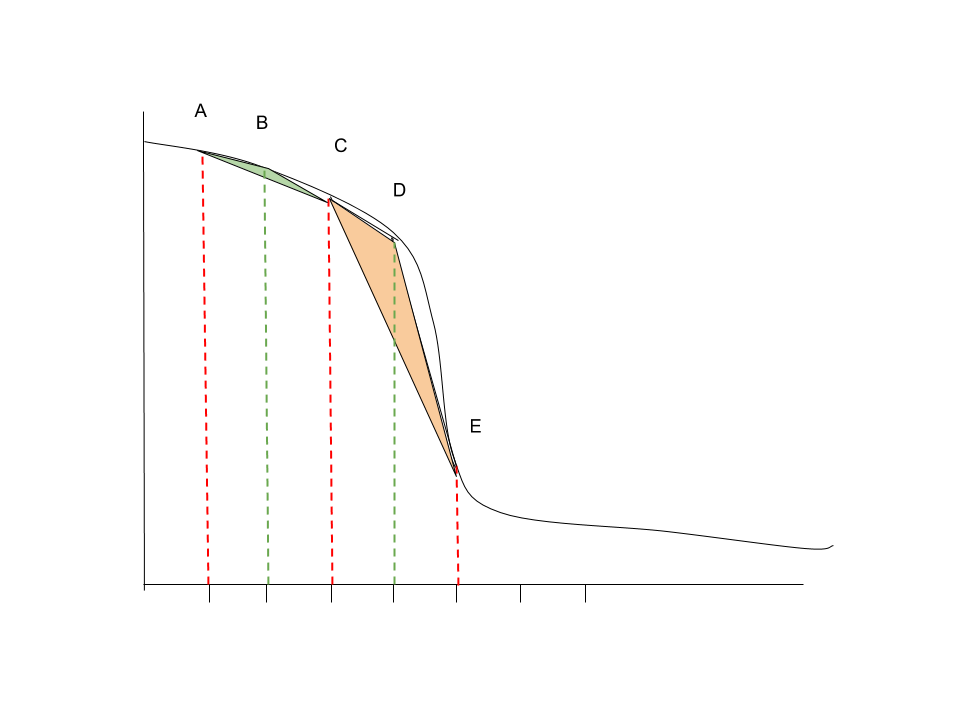
\includegraphics[width=\linewidth]{DROPBORINGLIN.png}
  \caption{A decreasing sampled signal.}
  \label{fig:boring}
\end{figure}

If we examine \ref{fig:boring} and imagine that there is a
time series which is sampled at points $A,B,C,D$, and $E$.
The colored triangles represent the ``error'' that
occurs if we compute the window ending between $A$ and $E$,
assuming that signal does not rise after that. It is
visually apparent that $B$ is a rather boring point compared
to $D$ in that the error that is produced by droppoing point
$B$ is much smaller than the error produced by dropping point $D$.

This observation is the heart of the algorithm: if the signal
never rises so that you run out of space, it is better to drop
the boring points.

A good data structure for this algorithm is a ring buffer
containing $R$ ``samples'', which contian both a value and a time,
and a ``client data field'' which contains the boringness.
By the observation of $MAXLIST$ we observe that
it behooves us to maintain the invariant that the elemets of this
buffer are ordered with increasing time and decreasing value.

The fundamental operation of a running algorithm is the addition
of a sample more recent than any in our ring, which we call
simple $INPUT$.

The algorithm $INPUT$ takes a current ring and a new sample $(v,t)$.
It returns an approximation to the maximum of the signal in a window of
duration $d$.

\begin{enumerate}
\item If $t-d$ is greater than the penultimate sample,
  drop the last sample from the ring.
\item Remove all elements from the ring which have a value
  less than $v$.
\item If the ring is full, drop the most boring element,
  computed from the head. Recompute the boringness of elements
  adjacent to the dropped element.
\item Add $(v,t)$ to the head of the ring.
\item If the ring contains 3 elements, assign a boringness
  to the element next to the head.
\item Return the linear interpolation of $(t-d)$ based
  on the last sample and the penultimate sample.
\end{enumerate}

Finding the most boring element may be done in constant time
by keeping a priority queue indexing the ring.

The function $BORING$ assigns a real number to an
element in the ring $B$ if it has a successor $C$ and predecssor $A$
in the ring. It takes the index of the element in the ring
and the ring as its argument. A small number is
considered ``more boring''. This is the area of
the triangle

$BORING(B,R)$:

\begin{enumerate}
\item Let $D = (A.t,C.v)$ and $E = (C.t,A.v)$. $ACDE$ is then
  a rectangle. Let $M$ be one-half the area of this rectangle.
\item Let $x$ = (B.t - D.t)(B.v - D.v)$.
  \tiem Return $M$ minus the area of the rectangle $BD$,
  which is $(B.v - D.v)(B.t-D.t)$  and the
  triangle $(B.t - A.t)(A.v-B.v))/2$, and
  the trinagle $(C.t-B.t)(B.v-C.v)/2$.
  \end{enumerate}






\bibliographystyle{unsrt}
\bibliography{pulseox}


\end{document}




